\chapter{Εισαγωγή}
\label{chap1}

%Εδώ αυτή κάνουμε μια γενική περιγραφή του χώρου εφαρμογής της διπλωματικής. Αναφέρουμε τα χαρακτηριστικά του χώρου και καταλήγουμε στα γενικότερα προβλήματα που αντιμετωπίζει ο χώρος. Η συζήτηση των προβλημάτων θα πρέπει να προϊδεάζει τον αναγνώστη για το τι θα προσπαθήσει να αντιμετωπίσει η διπλωματική, χωρίς ακόμα να αναφερόμαστε συγκεκριμένα στο αντικείμενο της διπλωματικής.
Είναι ευρεώς διαδεδομένο πως η ψηφιακή ενημέρωση βαδίζει πλέον με ραγδαίους ρυθμούς. Αμέτρητοι είναι σήμερα οι ιστότοποι και διαδικτυακές κοινότητες που σχετίζονται με όλες τις εκφάνσεις της καθημερινότητας, καθώς νέες εφαρμογές ενημέρωσης, οργάνωσης και επικοινωνίας αναδύονται στην ψηφιακή αγορά καθημερινά. Με μια αναζήτηση στο διαδίκτυο, ή με μια επισήμανση εντός της εφαρμογής, ο χρήστης μπορεί να ενημερωθεί για γεγονότα που τον ενδιαφέρουν, να δεχθεί ειδοποιήσεις για εκδηλώσεις που τον αφορούν, ή ακόμη και να προγραμματίσει το δρομολόγιό του, να υπολογίσει χρονικές και οικονομικές μεταβλητές και να σχεδιάσει το πλάνο του. Είναι λοιπόν ευνόητο το πρόβλημα που ανακύπτει από το παραπάνω φαινόμενο, σχετικά με την επικαιροποίηση και ενημέρωση της πληροφορίας που παρέχεται στο χρήστη. Παράγοντες όπως κυκλοφοριακή συμφόρηση, καιρικές αντιξοότητες, καθυστέρηση έναρξης μιας εκδήλωσης ή της άφιξης των συμμετεχόντων και άλλες αναπάντεχες εκβάσεις είναι αδύνατο να συνυπολογιστούν με κάποιον αλγόριθμο στις προαναφερθείσες εφαρμογές.

Από την άλλη, η απότομη στροφή των εφαρμογών και των μέσων κοινωνικής δικτύωσης γύρω από την ατομικότητα, έχει ως αντίκτυπο την αποδυνάμωση της συμμετοχής στο \textit{κοινωνικό γίγνεσθαι}. Πλέον είναι προτιμότερη η απομακρυσμένη έμμεση επικοινωνία με μέσα που τροφοδοτούν το χρήστη με εγωπαθή συμπτώματα και τον απομακρύνουν από την πραγμαματική έννοια της επικοινωνίας. Συχνό είναι επίσης το φαινόμενο εκμετάλλευσης της κοινωνικής προβολής για επαγγελματική ανέλιξη. Συνεπώς, γεγονότα  πολιτισμικού ενδιαφέροντος περνάνε σε δεύτερη μοίρα (βλ. Σχ \ref{socialmediausage}). 

Σαν αποτέλεσμα, τόποι κοινωνικού και πολιτισμικού περιεχομένου επισκιάζονται από αυτές τις εφαρμογές ``\textit{γίγαντες}'' (\selectlanguage{english}\textit{facebook, instagram, snapchat, twitter, tinder}\selectlanguage{greek} κλπ.). Εκδηλώσεις που χρήζουν προσοχής καταλήγουν να μην δέχονται την κατάλληλη προβολή. Είναι επομένως επιτακτική η ανάγκη ευαισθητοποίησης του χρήστη προκειμένου να δράσει υπερ του προσωπικού, αλλά ταυτοχρόνως και κοινωνικού οφέλους.   

\begin{figure}[!t]
	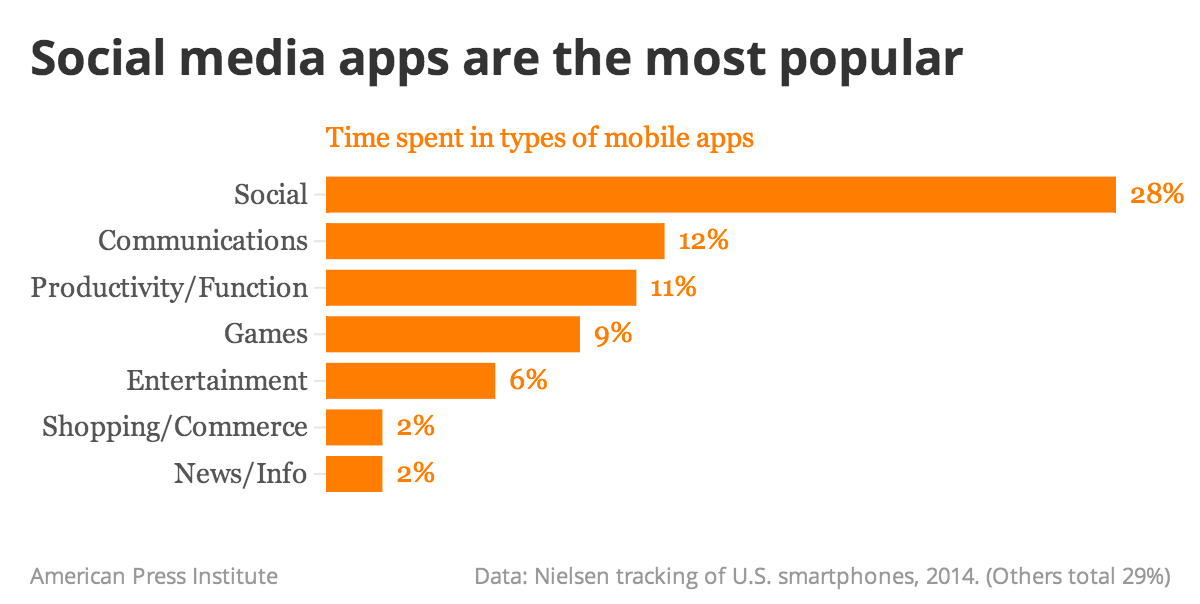
\includegraphics[scale=0.3]{figures/social-media-usage.png}
	\centering
	\caption{Οι χρήστες ξοδεύουν 14 φορές περισσότερο χρόνο χρησιμοποιώντας εφαρμογές όπως το \selectlanguage{english} \textit{facebook}\selectlanguage{greek}, έναντι εφαρμογών ενημέρωσης  (Πηγή: \cite{[AMP+14]})}
	\label{socialmediausage}
\end{figure}



\section{Αντικείμενο της διπλωματικής}

Εδώ αναφερόμαστε συγκεκριμένα στο τί θα κάνει η διπλωματική. Αναφέρουμε λεπτομερώς α) τα προβλήματα που θα λύσει (και που ήδη έχουν περιγραφεί γενικά στην προηγούμενη ενότητα), και β) πώς σκοπεύει να τα λύσει. 
Είναι σημαντικό κάποιος που θα διαβάσει την ενότητα αυτή να καταλάβει σε σημαντικό βαθμό τον σκοπό της διπλωματικής σας και τις τεχνικές δυσκολίες της, χωρίς να είναι αναγκαίο να δει όλα τα άλλα κεφάλαια. Η ενότητα αυτή θέλει πολύ προσοχή και καλύτερα να τη γράψετε αφού έχετε γράψει όλα τα υπόλοιπα κεφάλαια.

Το αντικείμενο με το οποίο καταπιάνεται το παρόν έργο, επικεντρώνεται στην σχεδίαση και την υλοποίηση μιας εφαρμογής, βασισμένη στην πρακτική ενεργοποίησης ενός ``\textit{πλήθους}'' ή μιας ομάδας, γνωστής και ως \textit{τακτική του πληθοπορισμού}. Η εφαρμογή που θα υλοποιηθεί θα υποστηρίζεται από \tl{iOS} πλατφόρμες σε όλες τις κινητές συσκευές. Η ανάπτυξη της εφαρμογής θα γίνει με τη χρήση των τελευταίων τεχνολογικών εργαλείων της αγοράς και θα ακολουθεί τις πιο σύγχρονες τάσεις που κυριαρχούν σήμερα στον ψηφιακό κόσμο.
\newline
\indent
 Πρωταρχικός στόχος της παρούσας εργασίας είναι να αναδείξει τις σύγχρονες τεχνολογίες που χρησιμοποιούνται σήμερα για την ανάπτυξη εφαρμογών, μέσα από τη σχεδίαση και υλοποίηση μιας καινοτόμου εφαρμογής. Ταυτοχρόνως, εισάγονται νέες ιδέες και τρόποι ανάδειξης τόπων πολιτισμικού περιεχομένου, μέσα από την ενεργοποίηση του κοινωνικού συνόλου. Οι χρήστες συμμετέχουν άμεσα σε πολιτισμικά δρώμενα, αναλαμβάνοντας ρόλους που έχουν άμεσο αντίκτυπο στην εικόνα του πολιτισμού. Μέσα από τη διαμόρφωση σχέσεων μεταξύ των χρηστών και της πολιτισμικής κληρονομιας, η εφαρμογή συνδράμει τόσο στην εξέλιξη της κοινωνίας, όσο και του πολιτισμού. 

\subsection{Συνεισφορά}

Η παρούσα διπλωματική εργασία σκοπό έχει να εμπλουτίσει τις δυνατότητες των χρηστών με πολιτιστικά ενδιαφέροντα. Χρησιμοποιώντας τις πιο πρόσφατες τεχνολογίες, θα προσφέρει μια ολοκληρωμένη εμπειρία μέσα από μια πλήρως λειτουργική και σύγχρονη εφαρμογή για πλατφόρμες \tl{iOS}. Η εφαρμογή θα δίνει στους χρήστες τη δυνατότητα να ενημερώνονται σχετικά με γεγονότα και εκδηλώσεις πολιτισμικού περιεχομένου, μέσα από τεχνικές βασισμένες στον πληθοπορισμό. Πρωταρχικό μέλημα είναι η προαγωγή του πολιτισμού, αξιοποιώντας τις δυνατότητες του διαδικτύου προς όφελος των χρηστών. Η λειτουργία της εφαρμογής θα σέβεται και θα προασπίζει την ασφάλεια του χρήστη, χωρίς να εμποδίζει την αλληλεπίδρασή του με το υπόλοιπο σύνολο, μέσα από την ανταλλαγή εντυπώσεων και το σχολιασμό γεγονότων. Επίσης, οι λειτουργικότητες της εφαρμογής μπορούν να αξιοποιηθούν από πολιτισμικούς οργανισμούς και φορείς για την βελτίωση του ρόλου τους μέσα από ανατροφοδότηση των χρηστών για μελλοντικούς σχεδιασμούς. 
\newline
\indent
Είναι κοινώς παραδεκτό πως ο πολιτισμός μπορεί να λειτουργήσει ως πεδίο σεβασμού της ετερότητας. H εφαρμογή μπορεί να διευκολύνει στο πεδίο αυτό, αναδεικνύοντας την αξία περιθωριοποιημένων ομάδων. Με τη δημιουργία μιας κοινής διεπιφάνειας χάρτη, ενοποιεί τις κοινωνικές ομάδες με κοινά ενδιαφέροντα και αναδεικνύει κοινούς τόπους. Συνδέει άτομα άγνωστα μέχρι πρότινος, άροντας όλα τα εμπόδια στην επικοινωνία και προωθώντας την διαλεκτικότητα, την αμοιβαιότητα και τον σεβασμό μνημείων πολιτισμικού ενδιαφέροντος. Επιπρόσθετα συμβάλλει στη δημιουργία μιας κουλτούρας του διαδυκτίου που σκοπό έχει την αναβάθμιση των χρηστών και όχι το κέρδος ή την εμπορευματοποίηση. 



\section{Οργάνωση του τόμου}
Η δομή της παρούσας εργασίας είναι οργανωμένη σε έξι επί μέρους κεφάλαια:

\begin{enumerate}
\item Στο \textbf{2ο Κεφάλαιο} παρουσιάζονται οι σημαντικότερες έννοιες, θεωρητικές αλλά και τεχνικές, οι οποίες είναι άρρηκτα συνδεδεμένες με το έργο και θα βοηθήσουν στην διαμόρφωση μιας σφαιρικής εικόνας. Επιπλέον παρουσιάζει σχετικές προσπάθειες που έχουν γίνει στο παρελθόν για συναφή αντικείμενα και θα βοηθήσουν στην ανάπτυξη της εφαρμογής. Τέλος, γίνεται αναφορά στις βασικές τεχνολογικές έννοιες που θα αξιοποιηθούν στην εφαρμογή, όπως \tl{REST APIs, OAuth, node} κλπ.
\item Στο \textbf{3ο Κεφάλαιο} αναλύονται οι λειτουργικές και μή λειτουργικές απαιτήσεις του συστήματος.Επίσης παρουσιάζεται η αρχιτεκτονική που θα ακολουθηθεί κατά την ανάπτυξη του συστήματος των διεπιφανειών του χρήστη, του εξυπηρετητή αιτημάτων και της βάσης δεδομένων.  
\item Στο \textbf{4ο Κεφάλαιο} επεξηγούνται οι τεχνικές σχεδίασης των διεπιφανειών της εφαρμογής και γίνεται μια εκτεταμένη ανάλυση του τρόπου σχεδίασης της κάθε οθόνης ξεχωριτσά. Επίσης παρατίθενται η λογική σχεδίασης του εξυπηρετητή αιτημάτων και της βάσης δεδομένων.
\item Στο \textbf{5ο Κεφάλαιο} αναλύεται λεπτομερώς η υλοποίηση του συστήματος. Αρχικά, γίνεται λόγος για τις λειτουργικότητες της εφαρμογής και τις τεχνικές με τις οποίες αυτές υλοποιούννται. Στη συνέχεια, γίνεται αναφορά στο τρόπο διαχείρησης των δεδομένων εντός της εφαρμογής. Τέλος, επεξηγούνται οι λόγοι επιλογής της πλατφόρμας προγραμματισμού. 
\item Στο \textbf{6ο Κεφάλαιο} γίνεται μια συνοπτική παρουσίαση του τελικού συστήματος, καθώς επίσης και μια ανάλυση των λειτουργικοτήτων που θα μπορούσαν να προστεθούν μελλοντικά στην εφαρμογή.  
\end{enumerate}




